%\documentclass{NECDC}
\documentclass[reqno]{lanl}

\usepackage[dvips]{color}
%\usepackage[xdvi]{color}
\usepackage[dvips]{graphics}
\usepackage{amsmath}

\definecolor{red}{rgb}{1,0,0}
\definecolor{blue}{rgb}{0,0,1}
\definecolor{green}{rgb}{0,1,0}
\definecolor{purple}{rgb}{1,0,1}

\definecolor{future}{rgb}{1,0,0}
\definecolor{verbatim}{rgb}{.5,.2,.8}

\newcommand{\splitcolor}[1]{\textcolor{blue}{#1}}
\newcommand{\futurecolor}[1]{\textcolor{red}{#1}}
\newcommand{\colorfuture}{\color{future}}
\newcommand{\colorverbatim}{\color{verbatim}}
\newcommand{\telegraphcolor}[1]{\textcolor{green}{#1}}

\newcommand{\comment}[1]{}


% If we aren't using NECDC style
\newenvironment{rmrkeywords}{%
  \setlength{\parindent}{2\parindent}
  {\bfseries Keywords:}}
  {\setlength{\parindent}{.5\parindent}}


%\NECDCDate{October 1998}

% Classification defaults to UNCLASSIFIED
%\NECDCClassification{\textcolor{red}{SECRET/RD}}


\newcommand{\del}{\ensuremath{\vec{\nabla}}}

\begin{document}

\title{Generic Programming in the SOLON Interface (U)}
\author{Randy M. Roberts}
\author{Geoffrey M. Furnish}
\author{Mark G. Gray}
\author{Shawn D. Pautz}
\address{X--TM, MS D409, Los Alamos National Laboratory, Los Alamos, NM
  87544}
\email{rsqrd@lanl.gov}
\email{furnish@lanl.gov}
\email{gray@lanl.gov}
\email{pautx@lanl.gov}

\subjclass{LA--UR--99--????}
\date{\today}

\keywords{generic programming, C++, radiation diffusion, 3T}

\maketitle

\begin{abstract}
Generic programming is not a new programming technique.
However,
until recently few programming languages contained the features necessary
for programmers to easily
and portably employ generic programming techniques 
in the construction of software.
With the ANSI standardization of C++ and the STL, the C++ Standard Template
Library, a language has become available that not only
contains these necessary features, but encourages their use.
This paper discusses the conceptual evolution of generic programming and
its application within the Solon 3T radiation package.~(U)
\end{abstract}

%\begin{rmrkeywords}
%  generic programming, C++, radiation diffusion, 3T
%\end{rmrkeywords}

\section{Introduction}

This paper traces the evolution of the software abstractions that have
led to generic programming.
The actual definition of generic programming is left until after the 
evolutionary process has been unfolded.
A short definition of generic programming, which attempts to maintain the
evolutionary theme, is the latest in a series of programming abstractions
that are used to organize and create computer programs with a high degree
of modularity, maintainability, efficiency and reusability.

After discussing the generic programming abstraction this paper will
demonstrate its use within the Solon 3T radiation package.
Generic programming is used within the Solon package as an aid to efficiently
incorporating Solon within any host application, perhaps a hydrodynamics
application.

\section{Early software abstractions}

\subsection{The subroutine abstraction.}
Much of the effort involved in software construction involves employing
abstractions that help organize and enable the reuse of software.
One of the earliest software abstractions, which has since become pervasive,
is the \emph{subroutine}.
With the 
advent of the subroutine code could be written and reused many times within
a program.
Particularly useful subroutines could even be placed into libraries,
and reused by many programs.

Here is an example of this early software abstraction, a subroutine
that can integrate a polynomial of any degree, between two integration
endpoints:
%
\colorverbatim \begin{verbatim}
double integratePolynomial(const double a[], int n, double x1,
                           double x2)
{
   // Code to integrate a polynomial of degree n,
   // between x1 and x2.
   // ...
}
\end{verbatim} \normalcolor
%
In this case the polynomial would be described by an array of coefficients,
$n$ long.
There would have to be agreement between
the subroutine author and the potential users of the subroutine
that the zeroth component of the array%
\footnote{C and C++ index arrays of length $N$
 beginning at $0$ and ending at $N-1$.}
would contain the constant coefficient, the first component contain
the linear coefficient, etc.

There are great benefits for writing such a subroutine.
In a program that will be integrating several polynomials between differing
integration bounds, writing this subroutine once saves programming time, 
and increases the understandability of the program.
In addition, having written and tested this subroutine once, you have limited
the number of potential bug ``nests,'' and have increased maintainability by
having only one subroutine to modify, if the need arises.

Another important aspect of this type of subroutine, which we will return
to later, is that it can be written to be very efficient for integrating
polynomials.
On the downside, this function can \emph{only}
 integrate polynomials, and only polynomials
specified precisely by an array of doubles as the coefficients and an integer
for the degree of the polynomial.
It cannot integrate a trigonometric function, 
nor even a \emph{complex} polynomial.

\subsection{Function Pointers.}
We can extend the subroutine abstraction by allowing the user
of the integration function
to specify as an incoming argument%
\footnote{In FORTRAN the same effect can be achieved by making the
argument ``external.''}
a pointer to a unary function that takes a double and returns a double.
This function pointer will be used to evaluate the function during the
integration process,
%
\colorverbatim \begin{verbatim}
typedef double (*pfunc_t)(double);
double integrateFunction(pfunc_t func, double x1, double x2)
{
   // Code to integrate the function, func.
}
\end{verbatim} \normalcolor
%
In this way you may now integrate a trigonometric function, although
you still cannot integrate a complex polynomial.

We now have a powerful mechanism for reuse.
\begin{itemize}
\item We have achieved reuse, in that we
  do not have to write a new subroutine for each integrand function.
  Any function that takes a double and returns a double is fair game for
  this integrator, including functions of our own construction.
\item Our
  integration routine is independent of the data structures used to represent
  the integrand functions.
  In the \texttt{integratePolynomial} function the data structure used to
  represent the polynomial was \emph{explicit} in the interface of the function,
  and could easily be in a form that is inconvenient for the client to use.
\end{itemize}

However, there are two main drawbacks to this, more general, approach.
\begin{itemize}
\item Specific integration routines, such as \texttt{integratePolynomial},
  can be written more efficiently, using the methods most suited to
  their specific tasks.
\item The pointer to unary function, \texttt{func}, cannot be inlined by
  the compiler.  Since \texttt{func} may be called many times, this could
  become costly.
\end{itemize}
%
Both of these problems can be overcome by the judicious use
of the generic programming abstraction.

\section{Generic programming}

\subsection{The integration example, continued.}
In regards to this somewhat contrived example of function integration,
generic programming techniques
can be used to address both of the drawbacks of using
function pointers.
This paper will focus on addressing the inlining issue.
Addressing the issue of using different methods for different classes
of integrand functions will require the use of more advanced
C++ language features.
%See~\mbox{Austern (1999)}
See~\cite{Austern99}
for information on using \emph{Tags}.

We begin by defining an integrator 
function templated on a \texttt{UnaryFunction}.
This function employs
(a very crude) trapezoidal algorithm to integrate the unary
function specified in its argument.
%
\colorverbatim \begin{verbatim}
#include <vector>
#include <functional>
#include <assert.h>

template<class UnaryFunction>
typename UnaryFunction::result_type 
  integrateFunctor(UnaryFunction functor,
                const typename UnaryFunction::argument_type &x1,
                const typename UnaryFunction::argument_type &x2)
{
   // Crude trapezoidal algorithm for demonstration

   return 0.5*(x2-x1)*(functor(x1)+functor(x2));
}
\end{verbatim} \normalcolor
%

The function \texttt{integrateFunctor} can be used with any class
for its \texttt{UnaryFunction} parameter that has
defined the nested types \texttt{result\_type} and \texttt{argument\_type}
as the correct return and argument types for its \texttt{operator()} method.
If the \texttt{operator()} method is an inlined method for this class
then the line of code with \texttt{functor(x1)+functor(x2)}
can be expanded with the inlined definition.
This can greatly increase the efficiency of the application.

The \texttt{MyPolynomial} class, below, is 
an example of a specific unary function object whose \texttt{operator()}
method evaluates the polynomial for a given argument.
%
\colorverbatim \begin{verbatim}
class MyPolynomial : public std::unary_function<double,double>
{
    std::vector<double> coefs;
    int                 order;

  public:

    MyPolynomial(const std::vector<double> &coefs_)
      : coefs(coefs_), order(coefs_.size())
    {
       // empty
    }

    // result_type and argument_type are defined in
    // std::unary_function

    result_type operator()(argument_type x) const
    {
       result_type p = coefs[order-1];
       for (int j=order-2; j>=0; j--)
          p = p*x + coefs[j];
       return p;
    }
};
\end{verbatim} \normalcolor
%
Notice that the class is publicly inherited from
\texttt{std::unary\_function<double,double>}.
The STL defines this class as a convenience, as it
defines the nested types \texttt{result\_type} and \texttt{argument\_type}.

This class acts as both an object and a function.
It has state, its coefficients, like an object, and it can be respond to the 
\texttt{operator()} like a function.

The function class and its use are tied together in this example.
%
\colorverbatim \begin{verbatim}
double useIntegrator()
{
   // load the polynomial coefficients

   double coefs_in[] = { 1.0, 2.0, 3.0, 4.0 };
   std::vector<double> coefs(coefs_in, coefs_in+4);

   // Create the polynomial functor

   MyPolynomial mypoly(coefs);

   // Integrate the polynomial from 1.0 to 3.0

   double result;
   result = integrateFunctor(mypoly, 1.0, 3.0);

   return result;
}
\end{verbatim} \normalcolor
%


\section{A Mesh-Type's evolution towards generic programming}

Solon uses the \texttt{MeshType} as the basis for its generic programming
strategy.
The classes that comprise Solon are each templated on a \texttt{MeshType}
parameter.
This class determines the data structures inherent in the mesh, as
well as determining the types of fields defined on the mesh.

In order to see the usefulness of this concept we will embark on the same
evolutionary journey for meshes and fields that we earlier took for the
function integrator, namely, from a \emph{flat data interface}, to
an \emph{object-based} design, to an \emph{object-oriented}
design, and finally to a \emph{generic programming} design.

\subsection{A flat data interface.}
Before programming languages enabled one to construct user-defined types
the only way to pass information about a mesh
was through direct access of the data that comprised the mesh.
The mesh might consist of the coordinates of the nodes,
the number of nodes and cells,
connectivity information, etc.
The fields defined on the mesh were simple one, two, or higher dimensional
arrays of data that were assumed to be related to the mesh in question.
Often the mesh and/or the fields were kept in common blocks.
When not kept in common blocks the mesh and fields were passed to the
subroutines that operated on them in the fashion as shown below.
%
\colorverbatim \begin{verbatim}
void solveP13T(const double coords[3][], ...,
               int ncells, double phi[], ...)
{
   // Solve cell-centered P1-3T equation on
   // mesh specified by coords, ncells, ...

   double *phiOld = new double[ncells];

   for (int i=0; i<ncells; i++)
      phiOld[i] = phi[i];

   ...

   delete [] phiOld;
}
\end{verbatim} \normalcolor

This approach has several disadvantages.
\begin{itemize}
\item This code has the data structure for the mesh and fields explicit in
  its interface.
\item Using arrays of intrinsics limits type safety.
\item A change in the mesh's data structure results in rewriting this
  function, and perhaps many others.
\item Only one ``type'' of mesh can be used in the package.
\item Parallelization strategy must be coordinated within this function,
  i.e.\ explicit calls to communication routines are required.
\end{itemize}

One of the few advantages of this approach is that the \texttt{solveP13T} 
function can be written to take full advantage of the mesh's data structure,
with great efficiency.

\subsection{An object-based Mesh class and field classes.}
We can mitigate the disadvantages of the flat data interface by encapsulating
and hiding the data structures for the mesh and fields.
We can construct a \texttt{Mesh} class and a \texttt{ccsf} -- 
cell-centered scalar field -- class and populate the members of the class with 
data that previously was exposed in the interface of the \texttt{solveP13T}.
The data for the mesh and fields can then only be accessed and manipulated 
by public interface methods, defined for their respective classes.

We would then rewrite \texttt{solveP13T} with \texttt{Mesh} and \texttt{ccsf}
objects as its arguments.
%
\colorverbatim \begin{verbatim}
void solveP13T(const Mesh &mesh, ccsf &phi, ...)
{
   // Solve cell-centered P1-3T equation on
   // mesh specified by "mesh"

   ccsf phiOld(mesh);
   phiOld = phi;
   ...
}
\end{verbatim} \normalcolor

This addresses the following disadvantages.
\begin{itemize}
\item The functions using meshes and fields no longer explicitly refer to
  the internal data structures in the interfaces.
\item Type safety is ensured by passing unique objects of types \texttt{Mesh}
  and \texttt{ccsf}.
\item A change in the mesh's or field's data structures does not require
  rewriting the function.
\item Parallelization can be coordinated within the methods of the mesh
  and field classes.
\end{itemize}

With carefully constructed and inlined methods on the mesh and fields we
can maintain the efficiency advantage found in the flat data interface.

\subsection{An object-oriented abstract mesh class and field classes.}
With the object-based approach
we are still left with the disadvantage that there can
only be one ``type'' of Mesh used in the package.
If we instead make the \texttt{Mesh} class an
\emph{abstract base class}, we can use the 
new \texttt{solveP13T} function with any class that is \emph{publicly derived}
from the \texttt{Mesh} class,
%see~\mbox{Booch (1994)}.
see~\cite{Booch94}.
The UML, Unified Modeling Language,
class diagrams for the \texttt{Mesh}
and \texttt{ccsf} classes are shown in figure~\ref{fig:mesh_uml},
%see~\mbox{Booch, et.al.\ (1999)} and~\mbox{Rumbaugh, et.al.\ (1999)}.
see~\cite{Booch99} and~\cite{Rumbaugh99}.

\begin{figure}
\center{\resizebox{.8\textwidth}{!}{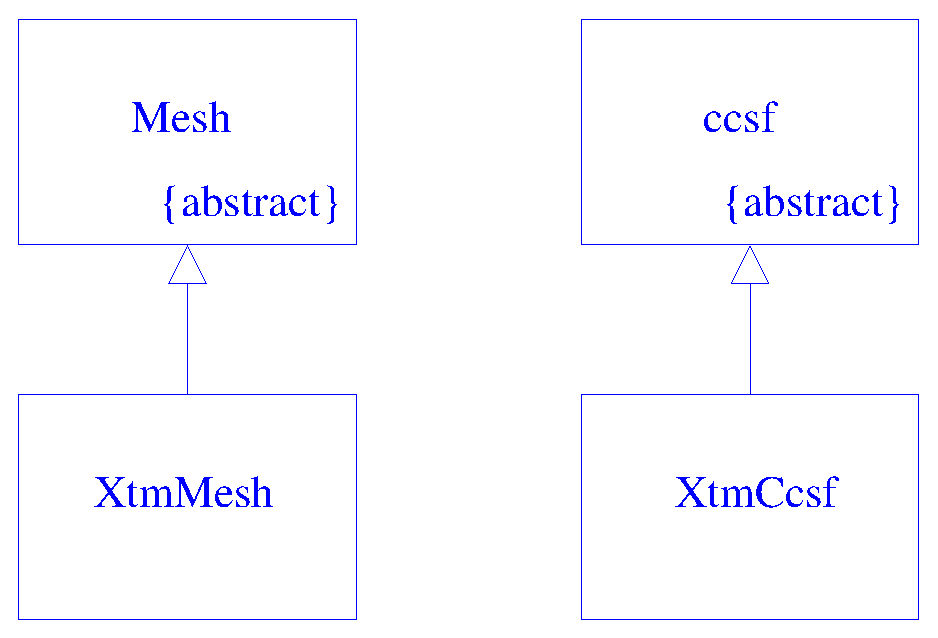
\includegraphics{mesh.uml.eps}}}
\caption{UML Inheritance hierarchy for mesh class
  and cell-centered field class.}
\label{fig:mesh_uml}
\end{figure}

In an object-oriented design all clients of mesh and field data use
references to the abstract base classes.
Any methods that are invoked on the base class references are forwarded
to the derived class methods through \emph{virtual functions},
 or \emph{virtual methods},
%see~\mbox{Cline, et.al.\ (1999)}.
see~\cite{Cline99}.
This process of invoking an unknown derived class's method through its
base class is called \emph{polymorphism}, or more specifically, \emph{runtime
polymorphism}.

With an object-oriented design we retain the advantages of 
encapsulization, type safety, and modularity that we gained with the
object-based design.
Unfortunately we sacrifice of the efficiency of inlined methods,
and incur extra overhead associated with the invocation
of virtual methods.

There is also a more insidious problem with this particular object-oriented 
mesh and field design.
We refer you to two lines from the code snippet for the object-based design,
%
\colorverbatim \begin{verbatim}
   ...
   ccsf phiOld(mesh);
   phiOld = phi;
   ...
\end{verbatim} \normalcolor
%
Now that the \texttt{ccsf} class has become abstract, you
are no longer allowed to create objects of that class, only objects of
classes publicly derived from the abstract class.
This limitation can be overcome through the use of \emph{abstract factory}
(aka. \emph{kit}), \emph{prototype},
or \emph{factory method} (aka. \emph{virtual constructor})
techniques,
%see~\mbox{Gamma, et.al.\ (1995)}.
see~\cite{Gamma95}.
So in reality, this is not a major limitation.

\subsection{A generic design using a Mesh-Type.}
With a generic programming design we can maintain the benefits of both the
object-based and object-oriented designs without the compromise of losing
efficiency that is gained with inlined mesh and field methods.

In a generic programming design we make use of \emph{genericity},
i.e.\ data access is through methods on objects of template argument
classes, e.g.\ \texttt{MeshType} in the following example.
The client method, \texttt{solveP13T}, does not know
the type of mesh and field classes with which it will be used.
This allows the client to be used with classes that need not be
related by a common base class as in the object-oriented design.
%
\colorverbatim \begin{verbatim}
template <class MeshType>
void solveP13T(const MeshType &mesh, MeshType::ccsf &phi, ...)
{
   // Solve cell-centered P1-3T equation on
   // mesh specified by "mesh"
   MeshType::ccsf phiOld(mesh);
   phiOld = phi;
   ...
}
\end{verbatim} \normalcolor
%
The actual classes used to instantiate the templated method must
meet certain requirements, or \emph{services}.
These services include specific nested type declarations, method signatures,
etc.
The sum of all of these services establish a \emph{concept} that candidate
classes must meet in order to be used with the client.
Any class that meets all of the requirements of the concept is considered
a \emph{model} of that concept.
%See~\mbox{Austern (1999)}
See~\cite{Austern99}
for more information about models and concepts,
and how they relate to generic programming.
See~\cite{Pautz99}
for more information about Solon's requirements for a mesh concept.

Any nested types within the concept are themselves concepts.
Any class that is a model of the former concept must have nested types
that are models of the latter concepts.
In our particular example any candidate model of our \texttt{MeshType}
concept must contain the nested \texttt{ccsf} type.
This \texttt{ccsf} class must itself be a model of our, as yet unnamed, 
cell-centered scalar field concept.

Since the model classes are used through template instantiation the
compiler can ``see'' the definitions of the methods for both the
model class and any nested classes declared by the model.
Therefore, the compiler may inline these methods, if the implementor
so chooses.
This means that there is more ``work'' for the compiler to perform,
thus degrading compilation times.
In our opinion this degradation of compilation times is small compared
to the benefits obtained by the use of this paradigm.

It should be noted at this point that generic programming is not
mutually exclusive with object-oriented programming.
In fact Solon makes use of both methods, where appropriate.
We use generic methods where efficiency is of greatest concern, and
runtime polymorphism (object-oriented methods) where efficiency is not
a concern.
Even when efficiency is a concern runtime polymorphism is used where
objects are manipulated only
via \emph{fat} methods, i.e.\ methods that perform
a lot of computational work.
Within these methods the compiler is able to ``see'' the code and may
perform any desired inlining.

The drawbacks associated with generic programming include
\begin{itemize}
\item the amount of up front work that is required to
      determine a good set of concepts for one's design
\item the multiplying number of instantiations required to
      span the use of the client code.
\end{itemize}

The first issue has to be addressed on a case by case basis by assessing
the requirements of one's customers, and using common sense.

The latter drawback is most keenly displayed by considering a client package
that is templated on $P$ parameter types (concepts).
Each of these parameter types has $M_{p}$ models that are desired to be
used within the entire program.
This requires that, somewhere within the code, there must be
$N = \prod_{p=1}^{P} M_{p}$ instantiations of that client package, and a
mechanism to choose from that set which instantiation to execute.
This multiplicity of instantiations can be mitigated through careful
use of factoring and runtime polymorphism,
again pointing to the need for a careful up front design.

\section{Generic programming in Solon}

\begin{figure}
\center{\resizebox{.8\textwidth}{!}{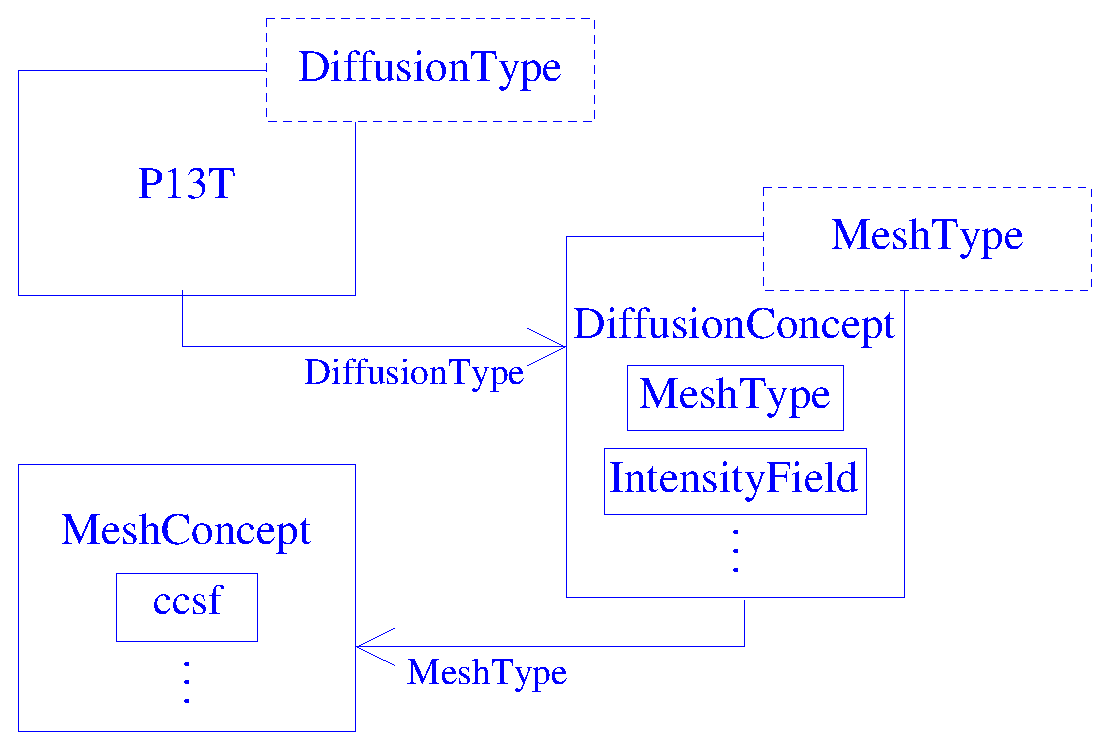
\includegraphics{p13t.uml.eps}}}
\caption{UML concept dependence for P13T class.}
\label{fig:p13t_uml}
\end{figure}

Although this paper has been motivating the construction of a \texttt{MeshType}
concept, Solon's principle class, \texttt{P13T}, is templated on a
\texttt{DiffusionType} template argument (concept), as shown in
figure~\ref{fig:p13t_uml}.
The \texttt{P13T} class calculates the coefficients of a P1 diffusion equation
\begin{equation}
  \label{eq:p1diffusion}
     - \del \cdot D \del \phi^{n+1} +  \bar{\sigma}^{a} \phi^{n+1}
                = \bar{Q}_{r} - \del \cdot \vec{F}'
\end{equation}
that are then passed to a model of the \texttt{DiffusionType}, to be solved.

The concept for the \texttt{DiffusionType}, i.e.\ \texttt{DiffusionConcept},
is templated on a
\texttt{MeshType} and exports the \texttt{MeshType} as a nested type definition.
The \texttt{DiffusionConcept}
also defines which physical entities are associated
with which field types.
For example, a cell-centered orthogonal diffusion solver would
specify that the radiation intensity be associated with a cell-centered
scalar field, i.e.\ \texttt{MeshType::ccsf}.
This association would be exported as a nested type definition of
\texttt{IntensityField} within the model of the \texttt{DiffusionConcept}.
Within \texttt{P13T} all fields are referenced by the nested type definitions
found within the \texttt{DiffusionType} template argument.

These fields can have differing representations depending on the host
code that uses the Solon package.
We currently have a \texttt{MeshType} based on our own \texttt{C4}
communications library.
In addition Julian Cummings, of the \emph{POOMA} project, has constructed
a \texttt{MeshType} that wraps the \emph{POOMA} (Parallel Object-Oriented
Methods and Applications) framework,
%see~\mbox{Reynders, et.al.}\ (1996).
see~\cite{Reynders96}.
We envision that any host that wishes to use Solon can create
a \texttt{MeshType} that wraps the host's data structures.

There are other projects that make use of our
\texttt{MeshType} concept.
Any host application that has constructed a \texttt{MeshType} for
Solon would be able to use the same \texttt{MeshType} with those other
applications, thereby amortizing the cost of the \texttt{MeshType}'s
development.

\begin{figure}
\center{\resizebox{.7\textwidth}{!}{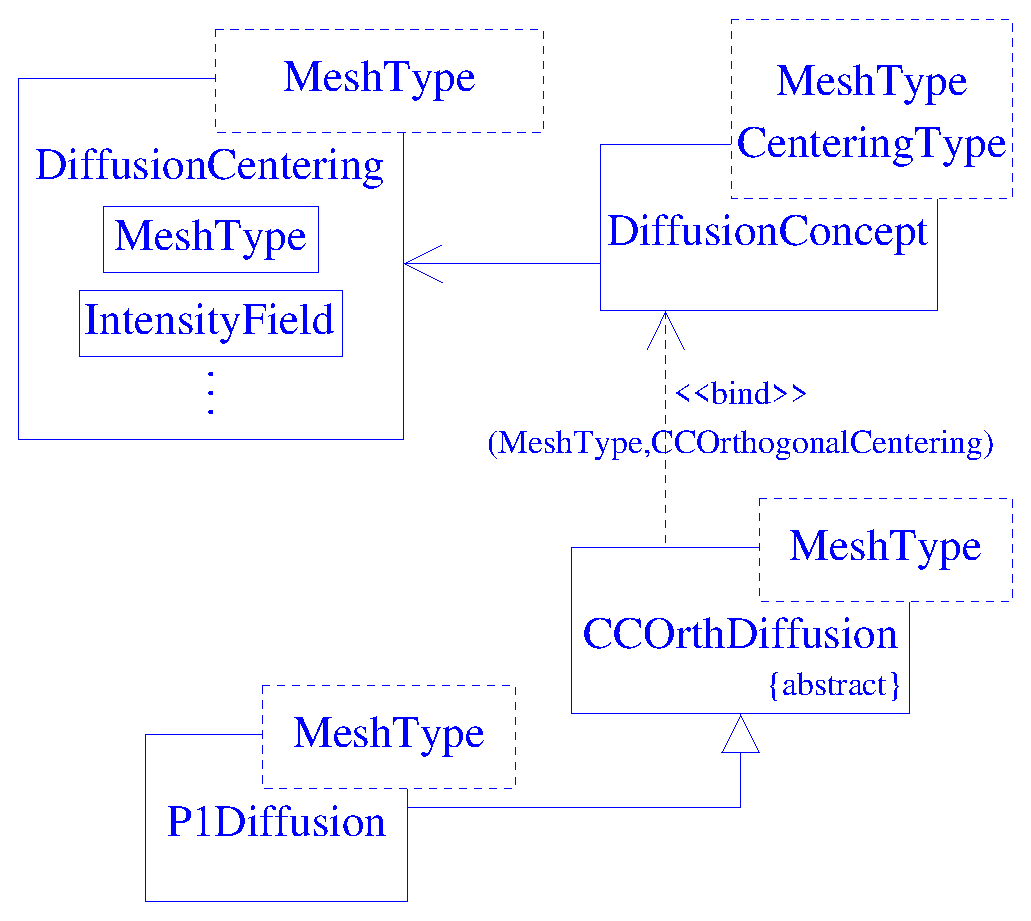
\includegraphics{diff.uml.eps}}}
\caption{UML dependence for diffusion classes.}
\label{fig:diff_uml}
\end{figure}

We have noticed one drawback to this current implementation of Solon, related
to the multiplicity of model instantiations that was mentioned above.
For every new diffusion solver method one would create a different
model of the \texttt{DiffusionConcept}.
This leads to an unnecessary number of template instantiations.

In our next design the mapping of the physical entities to their associated
fields will be factored out of the diffusion solver concept, into a replacement
\texttt{DiffusionCentering} concept.
Multiple diffusion solvers that use the same centering of physical entities
would use the same model of the \texttt{DiffusionCentering} concept.

The concept relationship for \texttt{P13T} would be identical 
with \texttt{DiffusionCentering} replacing 
\texttt{DiffusionConcept}.
In addition, particular diffusion solvers,
e.g.\ \texttt{P1Diffusion}, would publicly derive from a particular
instantiation of the \texttt{DiffusionConcept} on a
specific \texttt{DiffusionCentering},
e.g.\ \texttt{CCOrthogonalCentering}, as shown in 
figure~\ref{fig:diff_uml}.

When a new diffusion solver is introduced that uses a 
\texttt{DiffusionCentering} that has been previously instantiated,
the new diffusion solver would be chosen
totally through runtime polymorphism.
Since the interface to the diffusion solver is through fat methods,
there would be little effect on efficiency.

\section{Conclusion}

We have described the generic programming paradigm
and motivated its use.
Generic programming allows us the flexibility to interface with multiple
host applications.
This generic interface allows Solon to operate with meshes and fields using
data structures that are native to the host application, allowing increased
opportunities for inlining of field operations.
Generic programming enables  us to achieve this flexibility
and efficiency without sacrificing type-safety.

There is more effort up front in the design of our package, but we 
believe the results are worth the effort.
There is some effort at the back end in the construction of a host's
\texttt{MeshType}, but this effort would already be
required to interface a physics package into the host.
In addition, the cost of \texttt{MeshType} can be amortized if multiple
packages are to be integrated into the host code.

\bibliographystyle{apalike}

\bibliography{Solon}

%\section{References}
%
%\noindent
%Austern, M.H., \emph{Generic Programming and the STL: Using and Extending
%the C++ Standard Template Library,} (Addison Wesley, Reading, 1999). \\
%Booch, G., \emph{Object-Oriented Analysis and Design with Applications}, 2nd ed,
%(Benjamin/Cummings, Redwood City, 1994). \\
%Booch, G., et.al., \emph{The Unified Modeling Language User Guide}
%(Addison Wesley, Reading, 1999). \\
%Cline, M.P., et.al., \emph{C++ FAQ}, 2nd ed,
%(Addison Wesley, Reading, 1999). \\
%Gamma E., et.al., \emph{Design Patterns: Elements of Reusable Object-Oriented Software},
%(Addison Wesley, Reading, 1995). \\
%Reynders, J., et.al., POOMA: A framework for scientific simulation
% on parallel architectures., In Wilson, G.V., et.al.\ 
%\emph{Parallel Programming using C++}, pages 553--594, MIT Press, 1996. \\
%Rumbaugh, J., et.al., \emph{The Unified Modeling Language Reference Manual}
%(Addison Wesley, Reading, 1999). \\

\end{document}
